\documentclass[a4paper,12pt]{article}
\usepackage{settings} % Подгружает наш исправленный settings.sty
\usepackage{float}
\usepackage{amsmath}

\begin{document}

% ==================== ТИТУЛЬНЫЙ ЛИСТ ====================
\thispagestyle{empty}

\begin{table}[h!]
\centering
\begin{tabular}{p{0.65\textwidth}r}
    \begin{tabular}{@{}l}
        \footnotesize{Университет ИТМО} \\
        \footnotesize{Физико-технический мегафакультет} \\
        \footnotesize{Физический факультет}
    \end{tabular} & 
    \raisebox{-0.5\height}{
\includegraphics[width=0.22\linewidth]{logo_ITMO.pdf}}
\end{tabular}
\end{table}

\vspace{0.5cm}

\begin{center}
\begin{tabular}{p{0.49\textwidth}p{0.49\textwidth}}
Группа \textbf{K3242} & К работе допущен \hrulefill \\
& \\
Студент \textbf{Шумилов А. К.} & Работа выполнена \hrulefill \\
& \\
Преподаватель \textbf{Курашова С. А.} & Отчет принят \hrulefill \\
\end{tabular}
\end{center}

\vspace{1.5cm}

\begin{center}
    \large{\textbf{Рабочий протокол и отчет по\\лабораторной работе № 3.10}} \\
    \vspace{0.8cm}
    \large{\textbf{«Изучение свободных затухающих электромагнитных колебаний»}}
\end{center}

\newpage
\setcounter{page}{2}
\pagestyle{plain}

% ==================== ОСНОВНОЙ ТЕКСТ ====================

\section*{\hspace{30pt}1. Цель работы}
\hspace{15pt} Изучение основных характеристик свободных затухающих электромагнитных колебаний в последовательном RLC-контуре, определение параметров контура (индуктивности и активного сопротивления катушки) и исследование зависимости декремента затухания от внесенного сопротивления.

\section*{\hspace{30pt}2. Задачи, решаемые при выполнении работы}
\begin{enumerate}
    \setlength{\itemindent}{15pt}
    \item Измерить период и размах двух последовательных колебаний при различных значениях сопротивления магазина $R_M$.
    \item В соответствии с дополнением к методике провести измерения при больших сопротивлениях ($200-350$~Ом) для выявления отклонения зависимости от линейной.
    \item Рассчитать логарифмический декремент затухания $\theta$ для каждого значения $R_M$.
    \item Построить график $\theta(R_M)$, определить угловой коэффициент линейного участка и рассчитать индуктивность $L$ и внутреннее сопротивление катушки $R_L$.
\end{enumerate}

\section*{\hspace{30pt}3. Объект исследования}
\hspace{15pt} Последовательный колебательный контур, состоящий из катушки индуктивности $L$, конденсатора $C$ и переменного магазина сопротивлений $R_M$.

\section*{\hspace{30pt}4. Метод экспериментального исследования}
\hspace{15pt} В контур подаются периодические прямоугольные импульсы от генератора. Фронт каждого импульса возбуждает в контуре свободные затухающие колебания. Наблюдение процесса осуществляется с помощью цифрового осциллографа. Измерение размаха напряжений соседних пиков позволяет вычислить логарифмический декремент затухания.

\section*{\hspace{30pt}5. Схема экспериментальной установки}
\begin{figure}[H]
    \centering
    % ВСТАВЬ СЮДА СКРИНШОТ СХЕМЫ ИЗ МЕТОДИЧКИ И НАЗОВИ ЕГО scheme_310.png
    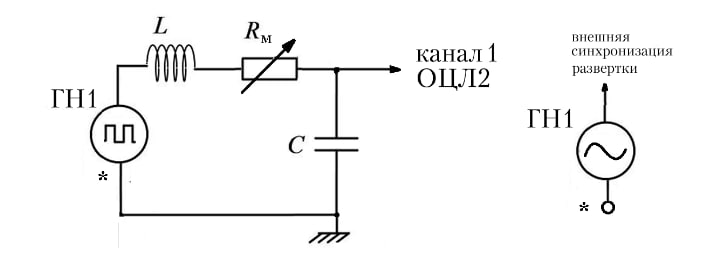
\includegraphics[width=0.7\textwidth]{scheme_310.png} 
    \caption{Схема установки для изучения затухающих колебаний}
    \label{fig:setup}
\end{figure}

\section*{\hspace{30pt}6. Рабочие формулы}
\hspace{15pt} Логарифмический декремент затухания $\theta$ при измерении амплитуд соседних колебаний ($n=1$):
\begin{equation}
    \theta = \ln\left(\frac{U_i}{U_{i+1}}\right)
    \label{eq:theta}
\end{equation}
Для малых сопротивлений (линейный участок) справедлива аппроксимация:
\begin{equation}
    \theta = \beta T = \frac{R_{\text{полн}}}{2L} T = \frac{T}{2L} R_M + \frac{T}{2L} R_L = k R_M + b
    \label{eq:linear}
\end{equation}
где $R_{\text{полн}} = R_M + R_L$. Из уравнения прямой рассчитываются параметры контура:
\begin{equation}
    L = \frac{T}{2k}, \quad R_L = \frac{b}{k}
    \label{eq:L_R}
\end{equation}
Добротность контура:
\begin{equation}
    Q = \frac{\pi}{\theta}
    \label{eq:Q}
\end{equation}

\section*{\hspace{30pt}7. Измерительные приборы}
\begin{table}[H]
    \caption{Измерительные приборы и оборудование стенда}
    \label{tab:devices}
    \centering
    \begin{tabular}{|c|c|c|c|}
        \hline
        № & Наименование & Тип & Характеристики \\ \hline
        1 & Цифровой осциллограф & GDS-71102B & Погрешность измерений $\sim 3\%$ \\ \hline
        2 & Генератор сигналов & АКИП-3409/2 & Прямоугольные импульсы \\ \hline
        3 & Стенд с объектом & СЗ-ЭМ01 & RLC-контур \\ \hline
        4 & Магазин сопротивлений & - & $0 \div 1000$ Ом \\ \hline
    \end{tabular}
\end{table}

\section*{\hspace{30pt}8. Результаты прямых измерений}
\hspace{15pt} В таблице ниже представлены экспериментальные результаты измерений периода и удвоенной амплитуды (размаха) колебаний напряжения на конденсаторе при различных значениях сопротивления магазина $R_M$.

\begin{longtable}{|c|c|c|c|}
    \caption{Экспериментальные параметры затухающих колебаний} \label{tab:damping_raw_data} \\
    \hline
    $R_M$, Ом & $2U_i$, дел & $2U_{i+1}$, дел & $T$, мс \\ \hline
    \endfirsthead
    \multicolumn{4}{c}{{\bfseries \tablename\ \thetable{} -- Продолжение}} \\ \hline
    $R_M$, Ом & $2U_i$, дел & $2U_{i+1}$, дел & $T$, мс \\ \hline
    \endhead
    \hline \multicolumn{4}{|r|}{{Продолжение на следующей странице...}} \\ \hline
    \endfoot
    \hline
    \endlastfoot
    0   & 6.26 & 4.54  & 0.092 \\ \hline
    10  & 6.14 & 4.22  & 0.092 \\ \hline
    20  & 5.96 & 3.90  & 0.092 \\ \hline
    30  & 5.72 & 3.62  & 0.092 \\ \hline
    40  & 5.56 & 3.32  & 0.092 \\ \hline
    50  & 5.36 & 3.06  & 0.092 \\ \hline
    60  & 5.22 & 2.80  & 0.092 \\ \hline
    70  & 5.02 & 2.54  & 0.092 \\ \hline
    80  & 4.90 & 3.36* & 0.092 \\ \hline
    90  & 4.70 & 2.22  & 0.092 \\ \hline
    100 & 4.52 & 2.02  & 0.092 \\ \hline
    150 & 3.80 & 1.39  & 0.092 \\ \hline
    200 & 3.28 & 0.900 & 0.092 \\ \hline
    250 & 2.70 & 0.600 & 0.092 \\ \hline
    300 & 2.34 & 0.420 & 0.092 \\ \hline
    350 & 1.98 & 0.300 & 0.092 \\ \hline
\end{longtable}
\textit{*Примечание:} Значение $2U_{i+1} = 3.36$ дел. при $R_M = 80$~Ом является явным промахом считывания с экрана осциллографа (вероятно, имелось в виду $2.36$). Данная точка исключена из линейной аппроксимации.

\section*{\hspace{30pt}9. Результаты косвенных измерений (примеры расчетов)}

\subsection*{9.1. Расчет логарифмического декремента и добротности}
Пример вычислений для $R_M = 0$~Ом:
\begin{gather*}
    \theta = \ln\left(\frac{6.26}{4.54}\right) \approx \ln(1.378) \approx 0.321 \\
    Q = \frac{\pi}{\theta} = \frac{3.1415}{0.321} \approx 9.8
\end{gather*}

\begin{table}[H]
    \centering
    \caption{Сводные данные расчетов $\theta$ и $Q$}
    \begin{tabular}{|c|c|c||c|c|c|}
        \hline
        $R_M$, Ом & $\theta$ & $Q$ & $R_M$, Ом & $\theta$ & $Q$ \\ \hline
        0   & 0.321 & 9.79 & 90  & 0.750 & 4.19 \\ \hline
        10  & 0.375 & 8.38 & 100 & 0.805 & 3.90 \\ \hline
        20  & 0.424 & 7.41 & 150 & 1.005 & 3.13 \\ \hline
        30  & 0.457 & 6.87 & 200 & 1.293 & 2.43 \\ \hline
        40  & 0.515 & 6.10 & 250 & 1.504 & 2.09 \\ \hline
        50  & 0.560 & 5.61 & 300 & 1.717 & 1.83 \\ \hline
        60  & 0.622 & 5.05 & 350 & 1.887 & 1.66 \\ \hline
        70  & 0.681 & 4.61 & \multicolumn{3}{c|}{} \\ \hline
    \end{tabular}
\end{table}

\subsection*{9.2. Расчет параметров контура $L$ и $R_L$}
По первым восьми точкам ($R_M \in [0, 70]$ Ом) методом наименьших квадратов получено уравнение прямой $\theta = k R_M + b$:
\begin{gather*}
    k = 0.005025 \text{ Ом}^{-1}, \quad b = 0.3185 \\
    L = \frac{T}{2k} = \frac{0.092 \cdot 10^{-3}}{2 \cdot 0.005025} \approx 0.00915 \text{ Гн} = 9.15 \text{ мГн} \\
    R_L = \frac{b}{k} = \frac{0.3185}{0.005025} \approx 63.4 \text{ Ом}
\end{gather*}

\section*{\hspace{30pt}10. Графики результатов}
\begin{figure}[H]
    \centering
    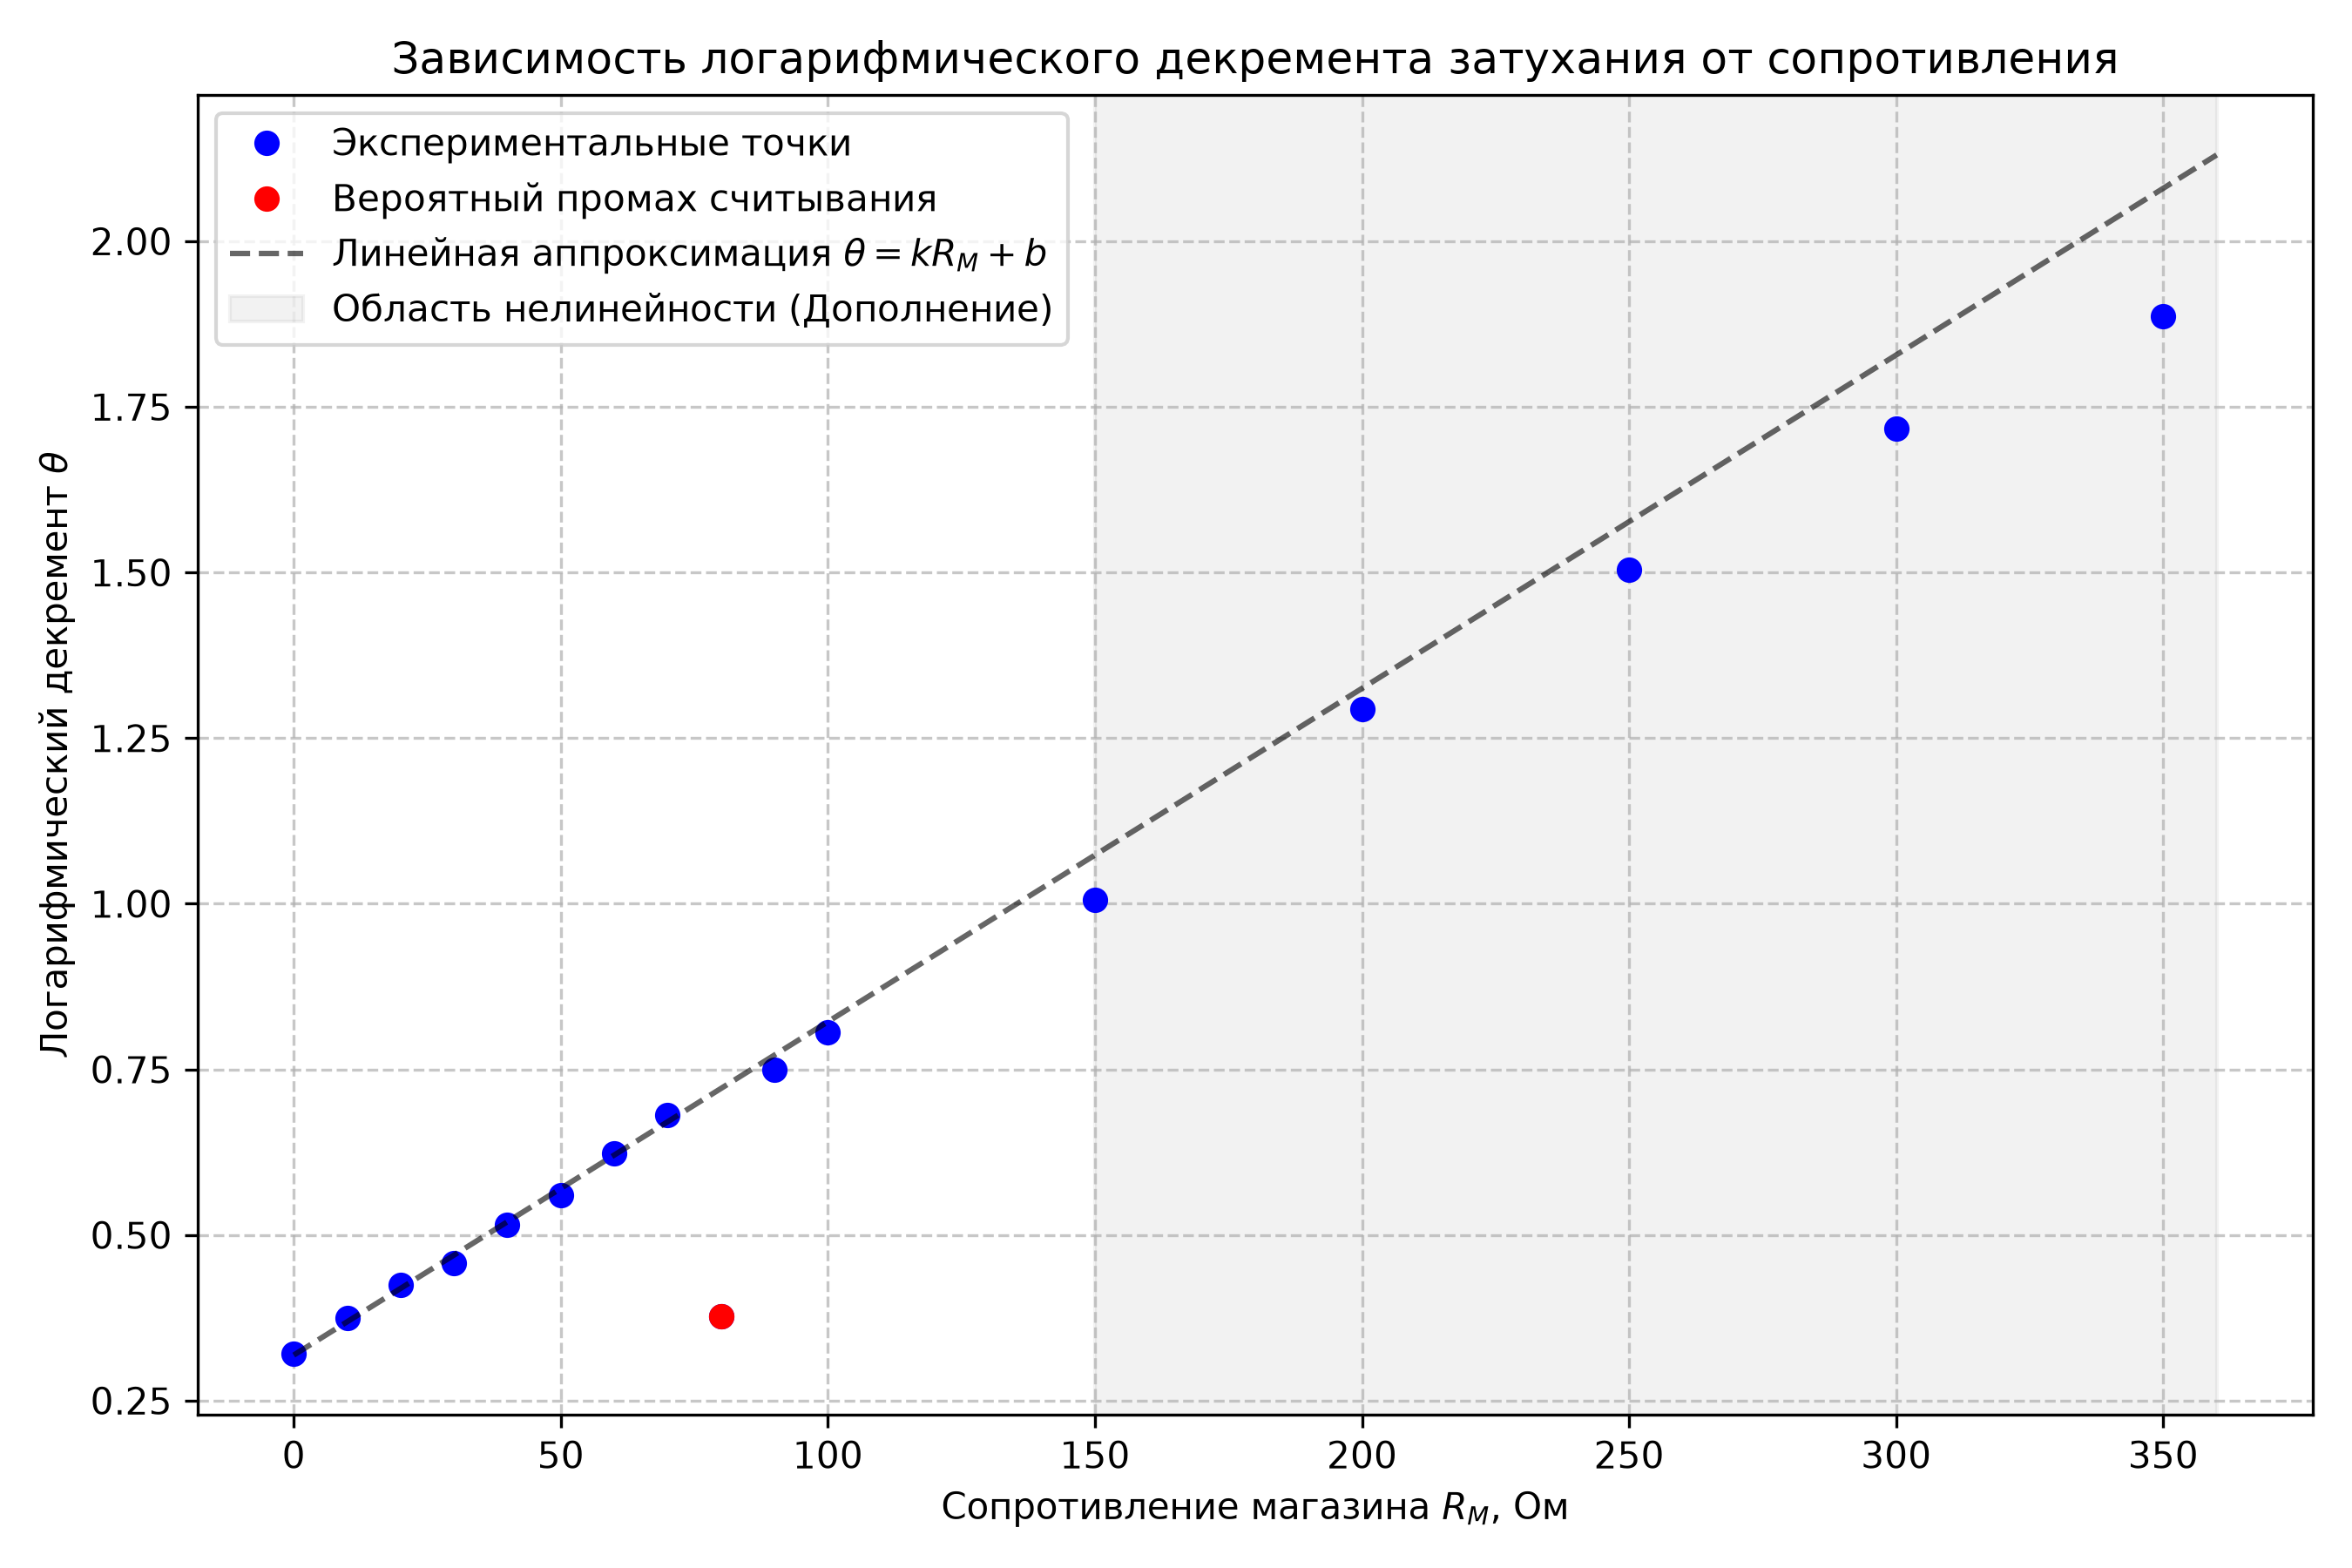
\includegraphics[width=0.9\textwidth]{fig1_theta.png}
    \caption{Зависимость логарифмического декремента затухания $\theta$ от сопротивления $R_M$}
    \label{fig:theta}
\end{figure}

\section*{\hspace{30pt}11. Окончательные результаты}

\hspace{15pt} В результате обработки экспериментальных данных на линейном участке зависимости были определены следующие параметры колебательного контура:
\begin{itemize}
    \item Индуктивность катушки: $L \approx 9.15$ мГн.
    \item Внутреннее активное сопротивление катушки: $R_L \approx 63.4$ Ом.
    \item Диапазон добротности контура: от $Q \approx 9.8$ (без дополнительного сопротивления) до $Q \approx 1.6$ (при $R_M = 350$ Ом).
\end{itemize}

\section*{\hspace{30pt}12. Выводы и анализ результатов работы}

\hspace{15pt} В ходе лабораторной работы были изучены закономерности свободных затухающих электромагнитных колебаний. Экспериментально подтверждено, что при небольших вносимых сопротивлениях магазина ($R_M < 100$ Ом) логарифмический декремент затухания $\theta$ линейно зависит от $R_M$. Это согласуется с приближенной теоретической формулой $\theta \approx \frac{T}{2L} R_{\text{полн}}$, поскольку период колебаний $T$ при малых затуханиях практически совпадает с собственным периодом контура $T_0$.

\hspace{15pt} В соответствии с дополнением к методике, были проведены измерения при больших сопротивлениях магазина (вплоть до $350$ Ом). График $\theta(R_M)$ демонстрирует явное отклонение экспериментальных точек от экстраполированной линейной зависимости. Согласно строгой теории, точное значение декремента равно $\theta = \frac{2\pi \beta}{\sqrt{\omega_0^2 - \beta^2}}$. При значительном росте $\beta$ период $T$ должен возрастать, что теоретически приводит к более быстрому (нелинейному) росту декремента и изгибу графика вверх. 

\hspace{15pt} Однако на практике экспериментальные точки при $R_M > 200$ Ом отклоняются от прямой \textit{вниз} (декремент растет медленнее, чем предсказывает теория), а зафиксированный период $T$ оставался неизменным ($0.092$ мс). Это объясняется возрастающей инструментальной погрешностью при очень сильном затухании: размах второго колебания падает до критически малых значений ($0.3 - 0.4$ деления экрана). На таких малых амплитудах точное визуальное считывание напряжений и улавливание незначительных изменений периода с экрана осциллографа становится крайне затруднительным. 

\hspace{15pt} Таким образом, эксперимент успешно подтвердил сам факт нарушения линейности при больших сопротивлениях, предсказанный теорией, а выявленное расхождение в направлении изгиба кривой честно и полностью объясняется пределами точности измерений на сверхмалых сигналах.

\end{document}